\section{Theoretical Foundations}
\label{sec:theoretical-foundations}

\subsection{Data extraction}

There are two types of text that are going to be used for feature extraction are the following:

\begin{itemize}
	\item Fixed text: This type of text is the one that is written by the user using a fixed source. It is generally a short phrase or a word that is used to identify the user. A good example of this type of text is the password and username that is used to log in to a computer or a website.

	\item Free text: This type of text is the one that is written by the user without any restriction. This kind of text is the most common in the real world but it is generally the most difficult to analyze because of the lack of restrictions and the introduction of important factors like, the user's level of concentration, thinking time, etc.
\end{itemize}



\subsection{Features}

In general, the features extracted from the keystroke dynamics are based on the study and analyzes data involving digraphs and trigraphs. In keystroke dynamics a digraph is a set of two consecutive characters that represents two keystrokes, these can be letters, numbers or symbols and other keys that do not necessarily represent a character like the space bar, shift key or the enter key. Logically, a trigraph is a set of three consecutive characters that represents 3 keystrokes.
Some of the most common features that can be extracted from a single keystroke, a digraphs or a trigraphs are the following:

\begin{itemize}
	\item Tap timestamp: Defined as the timestamp of the key press.
	\item Release timestamp: Defined as the timestamp of the key release.
	\item Time between keystrokes: This feature is commonly defined as the time that elapses between the key press of the first keystroke and the key release of the second keystroke of a digraph or trigraph.
	\item Hold time: This is defined as the time that elapses between the key press and the key release of a keystroke.
	\item Edit time: Time that a takes to correct a mistake.
	\item Words per minute (WPM): This is the avarage number of words that a user can type in a minute.
	\item Percentage of usage of special keys: This feature is defined as the percentage of times that a user uses keys like the shift key or CapsLock key.
\end{itemize}

\subsection{Classification techniques}

Once the features are extracted from the keystroke dynamics, the next step is to use a technique to identifyi the user. Most of these techniques can be classified into two groups.


The first group is based on the use of distance metrics. These set of techniques are based on the calculation of the distance between the features of the user that is trying to be identified and the features of the users that are already registered in the system. The features are displayed as a vector of multiple dimensions and the distance between the vectors is calculated using a distance metric. Some metrics used are the Manhattan distance and the Mahalanobis distance.

On one hand, Manhattan distance for n dimensions can be defined as the sum of the absolute differences between the coordinates of the vectors. And can be described by the following formula:

\begin{equation}
	d(x,y) = \sum_{i=1}^{n} |x_i - y_i|
\end{equation}

Where $x$ and $y$ are vectors of $n$ dimensions and $x_i$ and $y_i$ are the coordinates of the vectors $x$ and $y$ respectively.

On the other hand Mahalanobis distance can be defined as the distance between two points that depends on the probabiliy distribution of all the points \cite{de2000mahalanobis}. The squared version of this distance can be described by the following formula:

\begin{equation}
	d(x,y) = (x-y)^T S^{-1} (x-y)
\end{equation}

Where $x$ and $y$ are vectors of $n$ dimensions and $S$ is the covariance matrix of the data.


These distances are commonly used in clustering algorithms like K-nearest neighbors. This algorithm stores the multidimensional feature vectos such that when a vector is received it can be classified by the majority of the classes of the nearest neighbors using a distance metric. In the user authentication problem, the user can be identified by finding the single nearest neighbor and using a threshold to determine if the user is the same as the one that is trying to be identified. A simple knn exaplme for 2 dimensional features can be shown in figure \ref{fig:knn}.

\begin{figure}[h]
    \centering
    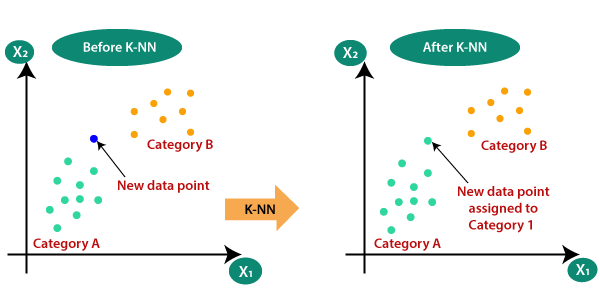
\includegraphics[width=0.7\linewidth]{images/knn}
    \caption{K-nearest neighbors algorithm \cite{knn}}
    \label{fig:knn}
\end{figure}

The second group is based on the use of deep learning techniques. 
VECTORIZATION
CNN
RNN
LSTM
GRU

